\chapter{文獻探討}


\section{品牌的定義}

根據各學者指出品牌的定義如以:

美國行銷學會(American Marketing Association,AMA)
對品牌的定義為:名稱 (Name)詞語(Term) 標記(Sign)象徵(Symbol )設計(design)\cite{AMA}

Sappington and Wernerfelt (1985) 品牌名稱是企業的一項貴重資產,可以提升消費者對
於產品的需求性,減少顧客的不確定感,且品牌名稱也被當成是對公司產品的品質保證。\cite{Sappington}

Farquhar (1989) 品牌是一個名稱、符號、設計或標誌,可以使一個產品增加的不僅是功能利益還有功能利益以外的價值。\cite{Farquhar}

Rao and Ruekert (1994) 品牌對於消費者而言是屬於產品的一部分,可視為傳遞產品品質訊息的媒介,而且往往是消費者購買決策的重要考量因素之一,具有增加產品價值的功能,而且可以提供產品一定的品質保證,降低消費者的搜尋成本及知覺風險。\cite{Rao}

Boyd, Walker, 和 Larreche (1995) 認為品牌的構成,成分一般可以細分為:
(一)品名(brand name):可以發聲唸出的部分。
(二)品牌標誌(brand mark):不能以言語表達的部分,例如符號、設計或獨特的包裝。 
(三)商標(trademark):法律上,專屬於某一個賣方的品牌或品牌的某部分。\cite{Boyd}

另外,根據 Laforet 和 Saunders (1994) 的實證研究,歸納出三種品牌導 向,六種品牌策略,這三種品牌導向所引發出的六個策略為:
(一)企業品牌導向
1.企業品牌策略:直接採用企業名稱作為產品品牌名稱。 
2.部門品牌策略:當企業跨足不同市場,單一企業名稱不敷使用時,不同部門採用不同附屬名稱 (subsidiary name) 作為產品品牌名稱
(二)產品品牌導向
1.個別品牌策略:各產品專屬品牌,不刻意突顯企業名稱,但在包裝上某 處仍會出現。
2.獨立品牌策略:各產品專屬品牌,但是刻意不揭露企業名稱,不希望消 費者知道是哪一家企業製造。
(三)混合品牌導向
1.雙重品牌策略:兩個或更多層級的品牌要素,組合而成產品品牌,而 且每個品牌要素的顯著性相等。
2.背書式品牌策略:同樣以兩種品牌要素組成品牌,但企業或家族品牌 作為背書之用,新產品的品牌較為顯著。\cite{Laforet}


\begin{table}[htb]
\caption{文獻整理}
\label{tab:PL1}
\centering
%\renewcommand{\arraystretch}{1.2} % 將表格行間距加大為原來的 1.2 倍
%\arrayrulewidth=1pt % 調整線條粗細為 1pt
%\tabcolsep=24pt % 調整欄間距為 24pt
%\begin{document}
\begin{tabular}[t]{|c|p{8.5cm}|p{2.5cm}|} % 第一欄位使用 sans serif 字族
\hline
學者&定義 & 年代 \tabularnewline
\hline
美國行銷學會 & 對品牌的定義為:名稱 (Name)詞語(Term) 標記(Sign)象徵(Symbol )設計(design)&  \tabularnewline
\hline
Sappington and Wernerfelt  &企業的品牌名稱是一個寶貴的資產,可以提升消費者對
於產品的需求性,減少顧客的不確定感,且品牌名稱也
被當成是對公司產品的品質保證。& 1985 (施瑩婕(2009)譯) \tabularnewline
\hline
Farquhar &品牌是一個名稱、符號、設計或標誌,可以使一個產品
增加的不僅是功能利益還有功能利益以外的價值。&1989 (施瑩婕(2009)譯) \tabularnewline
\hline
Rao and Ruekert &品牌對於消費者而言是屬於產品的一部分,可視為傳遞產品品質訊息的媒介,而且往往是消費者購買決策的重要考量因素之一,具有增加產品價值的功能,而且可以提供產品一定的品質保證,降低消費者的搜尋成本及知覺風險。&1989(施瑩婕(2009)譯)  \tabularnewline
\hline
 Laforet 和 Saunders&歸納出三種品牌導 :(一)企業品牌導向(二)產品品牌導向(三)混合品牌導向
&1994\tabularnewline
\hline
oyd, Walker, 和 Larreche&認為品牌的構成,成分一般可以細分為:(一)品名(brand name)(二)品牌標誌(brand mark)(三)商標(trademark)&1995\tabularnewline
\hline
\end{tabular}
\end{table}

\section{品牌知覺}
Aaker (1991) 將消費者對品牌的知覺品質定義為消費者對於某一 項品牌產品整體品質的認為水準,或消費者對在特定目的下相對於其他品牌, 對某品牌產品或服務全面品質的主觀滿意程度。\cite{Aaker1991}

kelle(1993)認為品牌認知是指在消費者記憶中較強的品牌聯想與連接。\cite{Keller1993}
將品牌知覺的衡量主要分成三種,敘述如下:
1. 屬性:消費者在消費之餘所認知的品牌是什麼、品牌有什麼。
2. 利益:指消費者個人價值。
3. 態度:指消費者對品牌整體的評價

Dawar and Parker(1994) 指出消費者挑選產品以品牌聲望為主要考量
Herbig and Milewica(1996) 正向的品牌聲望有助收益增加。
Kowallczyk and Pawlish(2002)公司聲望是影響消費者購買的因屬之一。
Veloutsou and Moutinho(2009)維持和提升公司聲望比強化消費者滿意度更重要
Priporas and Kamenidou(2011)品牌聲望佈警示品牌保證,也是行銷推廣的利器
\section{品牌行銷}

keller (1998)提出可以從四種角度說明品牌的意義與功能\cite{Keller1998}

1.品牌可以用圖案來辨別,可用來與競爭者來區別

2.品牌一致的保證與承諾,是消費者在購買或使用之前的感覺產品的價值與品質

3.品牌是可以自我投射形象,品牌個性的傳達

4.品牌是一組是有關產品的定位,代表一致性品質與功能性的集合,可作為消費者決策購買時的線索

Aaker (1996)認為品牌權益可分為:(1)品牌知名度 (Brand Awareness)、(2)品牌忠誠度 (Brand loyalty) 、(3)品牌知覺品質 (Brand perceived quality) 、(4)品牌聯想 (Brand Association)、(5)其他品牌專屬資產 (Brand Speciality Asset) 。\cite{Aaker1996}

    Keller (1998)亦詳細地指出,品牌權益實包含:(1)品牌鮮明度 (Brand Salience):可能會影響消費的判別難易度,(2)品牌績效 (Brand Performance):可以滿足消費者所需功能,(3)品牌形象 (Brand Image):在消費者心中產生對品牌抽象整體概念,(4)品牌判斷 (Brand Judgment) :消費者對於品牌理性層面的判定,(5)品牌情感 (Brand Feeling):消費者對品牌情感的概念與特性,或是社會認可的特徵,(6)品牌共鳴 (Brand Resonance):與消費者品牌關係的最高層次,是由品牌情感到具體行動購買的具體表現,例如主動參與及重複購買的行為忠誠度。\cite{Keller1998}

\begin{figure}[htbp]
\centering 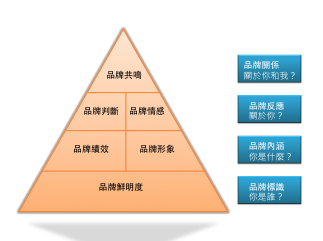
\includegraphics[%
  width=13cm,keepaspectratio]{images/keller2008}
\caption{\label{fig:keller}來自keller2008}
%(資料來源:本研究整理)
\end{figure}


\section{消費者行為}
早期的消費者行為通常都以消費者動機來當研究核心,隨著各位學者長年研究下來提出了許多相關理論的模式,但是現在研究後期主要都已決策的過程為主要核心

Schiffman&Kanuk(2003)瞭解消費者是如何進行決策,以支配可得資源 (時間、金錢、努力)於各種消費項目。這些決策 包括購買何種物品 (what)?為何而買 (why)? 何時購買 (when)?在哪裡購買 (where)?多常 購買 (how often)?以及使用 (use) 頻率。\cite{Schiffman}

Pratt(1974)消費者行為是只購買行動,其中購買的行動至 少包括四個因素:(1) 購買主體-購買者本身; (2) 購買物品或勞務;(3) 購買媒介-現金或支 付的承諾;(4) 決定購買的行動。\cite{Schiffman}

Walter&Gordon(1970)指人們在購買、使用產品或服務時的相關行為。\cite{Pratt1974}

林靈宏(2000)將消費者個體視為一個心理單位,消費者的價 值觀、知覺、學習、人格、動機、經驗、記憶、 認知、態度及涉入程度都會影響消費行為。\cite{林靈宏}

消費者決策行為模式有好幾種,其中較為完整且具系統性的模式架構的
是EKB Model(Engle, Kollat & Blackwell Model)。
Engel, Blackwell, and Kollat 等學者在 1968 年從消費者行為理論中,發展出了 EKB 模型 (Engel-Kollat-Blackwell Model, EKB Model),
在 EKB 模型中,可以分為四大部分:
\begin{enumerate}
\item輸入(Input):消費者所接受的外界訊息,其主要來自於兩方面:一是非行銷來源,如大眾傳播媒體或人際溝通管道;二是從行銷來源,如廠商的行銷活動。
\item資訊處理(Information Processing):資訊處理是經由刺激的接受、中斷與記
憶的儲存和稍後取用的過程,可分為展露(Exposure)、注意(Attention)、理
解(Comprehension)、接受(Acceptance)及保留(Retention)等五個步驟。
\item決策過程(Decision Process):決策過程可分為五個階段,是EKB模型中最 主要的部分,
此五個階段雖然是線性的過程,但卻可以反覆地回到之前的階段(Zellwegger 1997),此五個階段敘述如下:

a. 需求確認(Problem Recognition):是消費者決策過程中的第一個階段,當消費者認知到現實與理想狀態存在著差距時,就會意識到需求的存 在,而這些需求有可能會被外部的或內部的因素所觸發,比如:廠商的 促銷活動或者是個人的經濟狀況提升等等。

b. 資訊搜尋(Information Search):消費者在確認了需求動機後,就會開 始搜尋資訊,搜尋的範圍包括了記憶中的知識及外部的環境,前者稱為 內部搜尋,後者則稱為外部搜尋。

c. 選擇評估(Alternative Evaluation):當消費者取得了足夠的資訊後,即 會對可能的選擇方案加以分析與評估,來做為後續制訂購買決策的依 據。

d. 購買(Purchase):經過審慎的分析與評估後,消費者會從選擇方案中選 擇其一購買;消費者在這階段中,也必須決定從何處以及如何購買。

e. 購後行為(Post-purchase):消費者在使用或消費所選擇的商品或服務 後,會對其做出評估,以做為下此購買的參考。

\item影響決策變數(Variables Influence Decision Process):影響決策過程的變數可 分為兩部分:一為環境因素,包括文化、社會階層、個人影響、家庭與情境 等因素;二為個人差異,包括消費者資源、動機與涉入、知識、態度、人格、 價值觀與生活形態。
\end{enumerate}
\section{消費者行為理論(Consumer Behavior Theory)}
\subsection{EBK消費者行為定義}
消費者行為可以定義於:消費者在搜尋、評估、購買、使用和處理一項產品、服務、和理念(ideas)時表現的行為。\cite{EBK}
\begin{figure}[htbp]
\centering 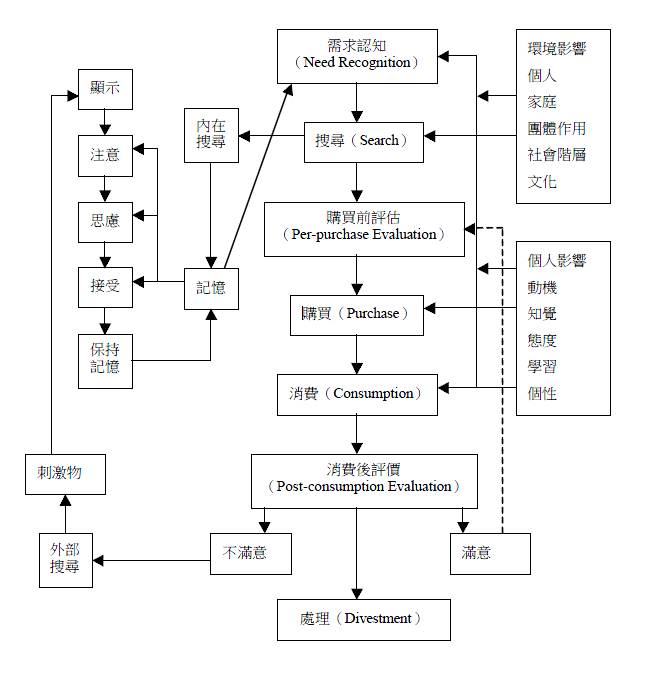
\includegraphics[%
  width=13cm,keepaspectratio]{images/ConsumerBehaviorTheory}
\caption{\label{fig:ConsumerBehaviorTheory}Engel, Blackwell and Kollat(1993)}
%(資料來源:本研究整理)
\end{figure}

\subsection{影響消費行為的心理因素}
消費者行為可以定義於:消費者在搜尋、評估、購買、使用和處理一項產品、服務、和理念(ideas)時表現的行為。\cite{林靈宏}
\begin{figure}[htbp]
\centering 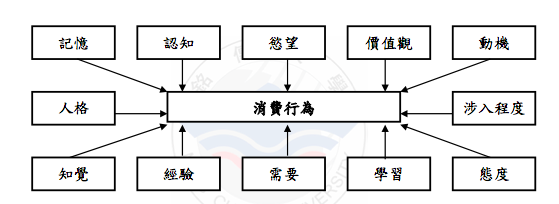
\includegraphics[%
 width=13cm,keepaspectratio]{images/影響消費行為的心理因素}
\caption{\label{fig:影響消費行為的心理因素}林靈宏 (2000),消費者行為學,台北:五南圖書出版公司。}
%(資料來源:本研究整理)
\end{figure}

\section{影響消費購買意願}
\subsection{購買意願之購買決策過程}
Engel, et al (2001) 認為,消費者決策過程的五個重要階段如圖~\ref{fig:Engel}

1.問題認知

購物過程開始時於消費者觀察自身需求與問題來源的認知 ;消費者在問題認知方面會受到外在因素影響(文化,人口統計變數,慘考群體)與個人因刺激,引起消費者產生動機

2.尋求

消費者在確定自己本身所需後,會根據自身問題或是所需來尋求相關資訊,以進行購物決策。一般的消費者收集資訊通常都分為兩種來源,內部搜尋與外部搜尋;消費者,通常會先從自身的記憶中搜尋所需的相關資訊,如過記憶中沒有相關記憶就會改以外部搜尋,獲得協助決策的相關資訊,外部搜尋的資訊如:家人,朋友,廣告,網路等。
           
3.方案評估

搜尋資料完後,就可以對所需要的選著方案做評估與最後的決策。通常消費者都是夠過各項評估的標準與尺度來評定購買的方案。

4.選擇

經過以上敘述方案評估過程後,消費者會以全部方案中選擇最適合的方案,並購買的行動。

5.結果 

當消費者購買產品後,因為本身對產品的期望結果與實際使用的結果,兩種之間的感覺受差異。
一般消費者購買的商品使用後心裡的感受主要有三中結果

符合期望:消費者使用購買的產品後的結果表現符合預期的期望,沒有特別好或壞的感覺

非常滿意:消費者使用購買的產品後的結果表現超過預期的期望,導致心裡的感覺很滿意

不滿意:消費者使用購買的產品後的結果表現低於預期的期望,導致心裡的感覺很不滿意的反應



\begin{figure}[htbp]
\centering 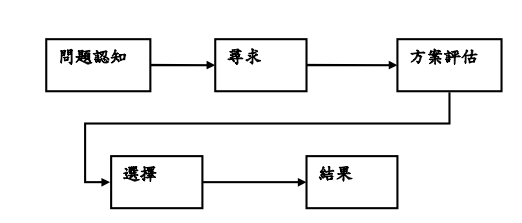
\includegraphics[%
  width=13cm,keepaspectratio]{images/Engel}
\caption{\label{fig:Engel}Engel, et al (2001)}
%(資料來源:本研究整理)
\end{figure}


\section{La jolla樂活雅}

公司簡介:

經營據點:台灣:台北市大安區光復南路446號七樓 
               美國:2231 N. 23rd St. Beaumont, TX 77706

 經營理念:富紳國際實業有限公司主要從事首飾及貴金屬零售業;擁有為數不少的客戶群。
最初,是由兩位業餘華裔設計師,自行創作手工珠寶藝品,由於設計風格獨特,大受消費者的歡迎及喜愛,總是供不應求。設計師們有鑑於手工飾品無法大量生產,又觀察到,在未來的飾品趨勢中,鈦飾品將取代金銀等貴重金屬,成為高級珠寶設計重要材質,因此決定發展鈦鍺飾品。

以生產設計鈦鍺精品為主的富紳國際,也接受客戶OEM及ODM訂單。舉凡項鍊、手鍊、戒指、袖扣等商品,並供貨給日本、美國等客戶及珠寶精品業者。
另外,富紳國際亦提供客製化服務,承接結合鈦飾品及頂級鑽石之客製化訂單,為消費者
提供獨一無二的商品訂製服務。

發展至今,富紳國際已擁有自己的設計師及協力生產工廠,從來圖打樣、來樣製作及專業生產一應俱全。專屬設計師群發揮豐富的創造力,賦與每一款設計精品獨創的理念,再結合老師傅精湛的珠寶鑲工技藝,精心打造每一分一毫細微處,提供國內外客戶最與眾不同、匠心獨具的頂級鈦鍺珠寶精品。

 企業文化:La Jolla品牌概念來自於美國加州。 La Jolla,源於西班牙文「珠寶」之意-「聖地牙哥的海洋之珠」,因為是西班牙文,所以唸法獨特,J的發音為H的氣音,唸作[ la-ho-ya](接近中文發音”拉荷亞)。La Jolla是一個位於美國加州San Diego的明媚小鎮。

在「陽光.沙灘.美麗海岸」的見證下,品牌創辦人遇見了”命中注定”的另一半,並於 La Jolla
小鎮買下了別具意義的定情戒,兩人互許真愛,相守一生。這份難能可貴的愛情,讓他們
決心將這份浪漫,轉化為璀燦迷人的健康概念純鈦飾品,將他們勇於追尋真愛的故事,透
過La Jolla精品,不斷的傳遞出去。

La Jolla品牌理念-Pure and  Trendy

Pure 材質純度嚴選 

Trendy 引領現代時尚精品風格 

「 La Jolla期許能結合藝術、自然、愜意美好的一切事物,以獨到細膩的品味設計、純鈦
的材質,帶來對生命最美好的感動。」 有別於一般市售的大眾化純鈦飾品, La Jolla
品牌創辦人堅持自我品味,精心打造一個具有現代時尚個性的純鈦精品。旗下專業設計師
更以獨創的設計理念,賦與每款飾品生命力,並結合老師傅細緻的鑲工手藝,極致講究每
一分每一毫細微的作工,呈現出純鈦精品的高雅質感及活力,演繹品味獨具的 La Jolla
純鈦精品新魅力。
 
品牌故事

有別於一般市售的大眾化鈦鍺飾品,La Jolla品牌創辦人CORA LIU堅持自我品味,精心打造一個具有現代時尚個性的鈦鍺精品。旗下專業設計師更以獨創的設計理念,賦與每款飾品生命力,並結合老師傅細緻的鑲工手藝,極致講究每一分每一毫細微的作工,呈現出鈦鍺飾品的高雅質感及活力,演繹品味獨具的La Jolla鈦鍺精品新魅力。

\begin{figure}[htbp]
\centering 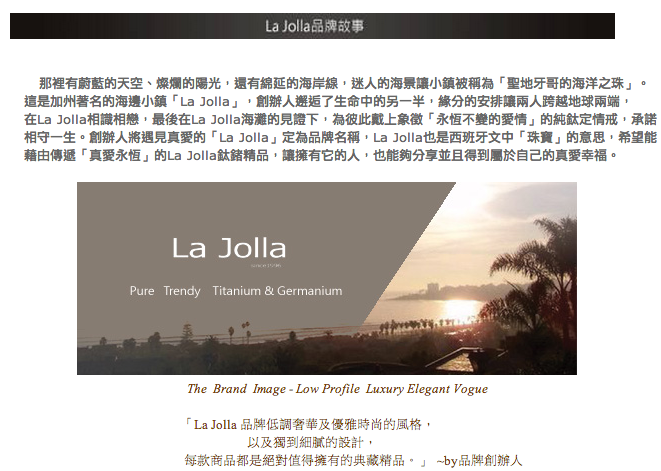
\includegraphics[%
  width=13cm,keepaspectratio]{images/LaJolla}
\caption{\label{fig:LaJolla}LaJolla樂活雅鈦鍺精品}
%(資料來源:本研究整理)
\end{figure}


